%Technical Review template made by Jeroen Hanselman for MaRDI (Mathematical Research Data Initiative)
%
% The template used for this technical review was adapted from the template made by Timmy Chan on https://github.com/TimmyChan 

%====================
% Packages and initialization
%====================
\documentclass[10pt]{article}
\usepackage[utf8]{inputenc}
\usepackage{graphicx}
\usepackage{pifont,xcolor}
\usepackage{amssymb}
\usepackage{TLCresume}
\usepackage{tikz}
\usepackage{parallel,enumitem}

%====================
% Colors and commands useful for the review
%====================
\definecolor{mardiblue}{RGB}{4,91,167}
\definecolor{mardiorange}{RGB}{208,102,49}

\newcommand{\mplus}[1][mardiblue]{
  \begingroup\leavevmode\color{#1}
  \setlength{\unitlength}{0.8em}
  \linethickness{.25em}
  \begin{picture}(1,1)
  \put(0,0.5){\line(1,0){1}}
  \put(0.5,0){\line(0,1){1}}
  \end{picture}
  \hspace{0.2em}
  \endgroup
}

\newcommand{\mminus}[1][mardiorange]{
  \begingroup\leavevmode\color{#1}
  \setlength{\unitlength}{0.8em}
  \linethickness{.25em}
  \begin{picture}(1,1)
  \put(0,0.5){\line(1,0){1}}
  \end{picture}
  \hspace{0.2em}
  \endgroup
}

\makeatletter
\newcommand*{\radiobutton}{
  \@ifstar{\@radiobutton0}{\@radiobutton1}
}
\newcommand*{\@radiobutton}[1]{
  \begin{tikzpicture}
    \pgfmathsetlengthmacro\radius{height("X")/2}
    \draw[radius=\radius] circle;
    \ifcase#1 \fill[radius=.6*\radius] circle;\fi
  \end{tikzpicture}
}
\makeatother

%====================
% Title of paper and authors
%====================

%====================
%====================
% FOR REVIEWERS TO FILL OUT (PART 1 of 12)

% Here you can write down the title of the paper and the names of the authors.
%====================
%====================
\def\titleofpaper{Algorithm to compute the number of carrots needed to complete a proof}   % <- Edit this
\def\authors{Jeroen Hanselman and Mardi the Math bunny}  % <- Edit this

%====================
% Review Header
%====================

\RequirePackage{fancyhdr}
\fancypagestyle{fancy}{%
\fancyhf{}
\lhead{



\textbf{Title: }\titleofpaper\\
\textbf{Author(s): }\authors  \\
\textbf{} \\
\textbf{Date: }\today\\ 
	    } 
	\chead{%
	    \centering {\huge \textbf{Technical review}} \\ %
	    }%
	    
\rhead{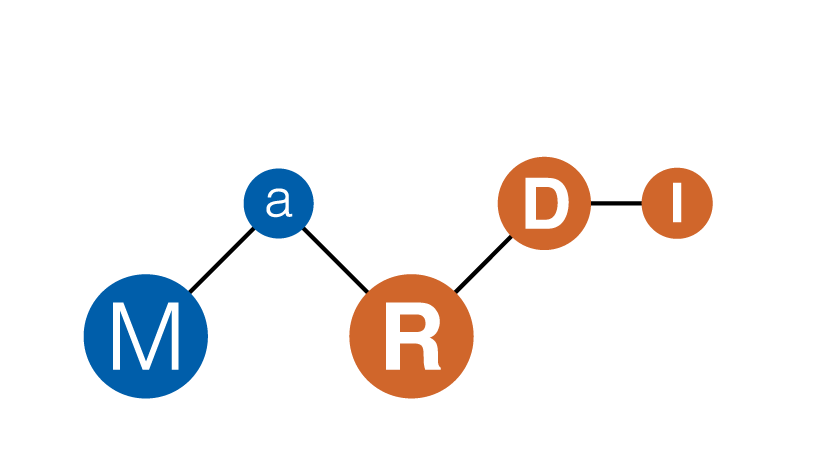
\includegraphics[scale=0.7]{Mardi.png}}
\renewcommand{\headrulewidth}{2pt}% 2pt header rule
\renewcommand{\headrule}{}
}
\pagestyle{fancy}

\setlength{\headheight}{150pt}
\setlength{\headsep}{5pt}

\begin{document}


%====================
% Sections of the review
%====================
\section{Basic Info}
%====================
% Basic Info
%====================
% Here you can indicate which files were included with the paper.
\begin{minipage}{0.30\textwidth}
\noindent\parbox[t]{1.2in}{\raggedright%
\vspace{0.5em}
\textbf{Files provided}

%====================
%====================
% FOR REVIEWERS TO FILL OUT (PART 2 of 12)

% For each item in the bottom list, there are two possbilities:
% -  a [\square] which will show up as an empty box [ ]
% - a [\boxtimes] which will show up as a crossed of box [x]
% Comment out (using %) whatever type of file is not included in the repository.
% If there are any types of files included in the list that are still important to mention, feel free to add
% the type of file to the list.
%====================
%====================

\begin{itemize}[topsep=0pt,itemsep=-2pt,leftmargin=13pt]
\item[$\square$] Source Code   % <- Edit this
%\item[$\boxtimes$] Source Code

\item[$\square$] Notebook
%\item[$\boxtimes$] Notebook

\item[$\square$]  Examples
%\item[$\boxtimes$] Examples

\item[$\square$] Docker file/VM
%\item[$\boxtimes$] Docker file/VM
\end{itemize}

\vspace{0.5em}
}%
\parbox[t]{1.2in}{\raggedright%
\vspace{1em}
\begin{itemize}[topsep=6pt,itemsep=-2pt,leftmargin=13pt]
\item[$\square$] Documentation   % <- Edit this
%\item[$\boxtimes$]  Documentation

\item[$\square$]  Computed data
%\item[$\boxtimes$] Computed Data

\item[$\square$] Files that verify computed data
%\item[$\boxtimes$] Files that verify computed data
\end{itemize}
\vspace{0.5em}
}
\end{minipage}%
\hfill
%
%====================
%====================
% FOR REVIEWERS TO FILL OUT (PART 3 of 12)
%
% Here you can list all the information about what software and hardware was used to perform the review. 
% To do so, replace the part behind  \textbf{bolded text:} & &  
%
% Programming languages can contain any langages you used as well as version information (if relevant), for example
% C, C++, Python 3.13.1, Julia v1.11.4. You can write N/A if there were no basic programming languages involved.
%
% Standard Software used can contain common Software packages for mathematics, for example
% Magma V2.27-8, SageMath v10.5, Oscar v1.3.1,  Maple 2024, Mathematica v.13.1, CoCoA 5, etc. You can write N/A if there was no standard software involved.
%
% System specs should contain, the OS, the processor, the amount of RAM memory on your system and any other relevant information.
%
%====================
%====================
\begin{minipage}{0.6\textwidth}
\begin{tabular}[t]{p{13em} p{1em} p{17em}}
\textbf{Programming languages:} & &  N/A \\   % <- Edit this
\textbf{Standard software used: }& &  Magma V2.27-8   \\  % <- Edit this
\textbf{System specs used for review :}& &  Ubuntu 22.04.1 with Intel i7-7700 processor, 4 cores @ 3.60GHz, 32GB RAM \\  % <- Edit this

%====================
%====================
% FOR REVIEWERS TO FILL OUT (PART 4 of 12)
% Here you can descrobe the version of the code you reviewed and where you downloaded it from.

% To do so, replace the part behind  \textbf{bolded text:} & &  
% In case the code is spread across multiple repositories, you could split the version and download information in multiple instances and use some keyword to distinguish between them. In case there is a Magma implementation and a Sage implementation, one could, for example, write: 

% \textbf{Version reviewed (Sage): v0.1.3 of the package}
% \textbf{Version reviewed (Magma): No version numbering. Files reviewed were last changed on the 11th of March 2024\\ }
% \textbf{Downloaded from: (Sage) }& &   \url{https://github.com/fakegithub/MathBunnyMadness} \\
% \textbf{Downloaded from: (Magma) }& &   \url{https://github.com/fakegithubforothercode/MathBunnyMadness} \\

\textbf{Version reviewed:}& &  No version numbering. Files reviewed were last changed on the 11th of March 2024\\  % <- Edit this
\textbf{Downloaded from: }& &   \url{https://github.com/fakegithub/MathBunnyMadness} \\  % <- Edit this

\end{tabular}
\end{minipage}%

\section{Importance of software in the paper}
%====================
% Importance
%====================

%====================
%====================
% FOR REVIEWERS TO FILL OUT (PART 5 of 12)

% Here you can indicate the role the code plays in the paper. Depending on what this is the focus of the review might be a bit different.  
% Common roles are:
% - The paper explains a new algorithm capable of computing things we were not able to compute before
% - The paper presents an algorithm that is claimed to be better than existing algorithms
% - The paper discusses a database of mathematical objects
% - The code is used to compute examples included in the paper
% - The code is used to do computations as part of a proof

% But it isn't necesarry to stick to one of these descriptions

%====================
%====================

The repository contains the implementation of the algorithms and the results of the computations described in the paper.\\  % <- Edit this

\section{Reproducibility (Installation)}
%====================
% Installation
%====================

%====================
%====================
% FOR REVIEWERS TO FILL OUT (PART 6 of 12)

% Here everything that has to with with installing the software can be written. 
% To do so, replace the text next to "% <- Edit this"
% To use the symbols (blue plus for a positive aspect, red minus for a negative minus) you can comment out their respective lines with %.

%====================
%====================
% 

\begin{tabular}[t]{p{15 em} p{1em} p{35em}} 
\textbf{License:}  & & 
%\mplus
\mminus 
No license found\\  % <- Edit this

\textbf{Availability: }& & 
\mplus 
%\mminus
The files were uploaded to GitHub \\ % <- Edit this

\textbf{Readme:} & & 
\mplus 
%\mminus
The repository contains a Readme explaining the contents of the Github. \\ % <- Edit this

\textbf{Installation:} & & 
\mplus 
%\mminus
Straightforward. \\ % <- Edit this
\end{tabular}


\section{Installation steps taken}
%====================
% Installation Steps
%====================

%====================
%====================
% FOR REVIEWERS TO FILL OUT (PART 7 of 12)

% Here you describe what steps you took to try to install the software. This can be especially helpful for the authors when you fail to install the software as it may allow them to reproduce the problem and fix it. 
% To do so, edit add an \item in the itemized environment for every step you took.

% If there are multiple pieces of software included in the paper, you can split the installation steps into separate parts and label them, e.g.

%\textbf{Magma Code:}
%\begin{itemize}
%\item Step 1
%\item  Step 2
%\end{itemize}

%\textbf{Sage Code:}
%\begin{itemize}
%\item Step 1
%\item  Step 2
%\item Step 3
%\end{itemize}

%====================
%====================
% 

\textbf{Code:}
\begin{itemize}
\item Cloned \verb|https://github.com/MaRDItheMathbunny/MaRDICode| from GitHub  
%\item  Step 2
%\item Step 3
%\item  etc.
\end{itemize} % <- Edit this

\section{Reproducibility (Records of setup)}
%====================
% Records of setup
%====================


%====================
%====================
% FOR REVIEWERS TO FILL OUT (PART 8 of 12)

% Here you write down whether the authors wrote down the specs of their system or OS that they used to produce their results. This is more important when the authors have code that takes a long time to run or when they compare their algorithm with other algorithms.
% To do so, replace the text next to "% <- Edit this"
% To use the symbols (blue plus for a positive aspect, red minus for a negative minus) you can comment out their respective lines with %.

%====================
%====================
% 



\begin{tabular}[t]{p{15 em} p{1em} p{35em}}
\textbf{Specification of CPU:}& & 
%\mplus
\mminus 
Did not find what CPU was used. \\  % <- Edit this

\textbf{Specification of Memory:}& & 
%\mplus
\mminus 
Did not find the amount of memory used. \\  % <- Edit this

\textbf{Specification of OS/software used:}& & 
%\mplus
\mminus 
Did not find which Magma version was used. \\  % <- Edit this

\textbf{References and citation: }& & 
\mplus 
%\mminus 
Magma is cited. The other packages the software builds on or depends on are properly cited.\\  % <- Edit this
\end{tabular}

\section{Reproducibility (Running the code)}
%====================
% Reproducibility
%====================

%====================
%====================
% FOR REVIEWERS TO FILL OUT (PART 9 of 12)

% % Here you describe whether you were able to run the code that was provided. You can furthermore mention any errors that showed up.

% To do so, replace the text next to "% <- Edit this"

% To quote error messages or parts of the code one could use the verbatim environment:  \begin{verbatim} CODE \end{verbatim}
% To use the symbols (blue plus for a positive aspect, red minus for a negative minus) you can comment out their respective lines with %.

% If there are multiple pieces of software included in the paper, you can split the evaluation of the reproducibililty into separate parts and label them, e.g.

%\textbf{Magma Code:}
%\begin{itemize}
%\item Step 1
%\item  Step 2
%\end{itemize}

%\textbf{Sage Code:}
%\begin{itemize}
%\item Step 1
%\item  Step 2
%\item Step 3
%\end{itemize}

%====================
%====================
% 

\begin{tabular}[t]{p{15 em} p{1em} p{35em}}

\textbf{Code:} & & 
\mplus 
%\mminus 
The code seems to run fine. It does give a small error however: \begin{verbatim}
In file "Carrot.m", line 587, column 9:
>> bunny := [ 0, 0, 0];
\end{verbatim}\\ % <- Edit this

\end{tabular}

\section{Correctness and Reliability}
%====================
% Correctness and Reliability
%====================

%====================
%====================
% FOR REVIEWERS TO FILL OUT (PART 10 of 12)

% In this section you can indicate how convinced you are that the code does what is claimed in the paper. Things that might make results more convincing are, for example, trying out different inputs, test files written by the authos or multiple implementations in different systems. But these are not strictly necessary. This section is mostly about if the output coincides with what was claimed and if the algorithms seem to be doing the correct thing.

% To do so, replace the text next to "% <- Edit this"

% To quote error messages or parts of the code one could use the verbatim environment:  \begin{verbatim} CODE \end{verbatim}
% To use the symbols (blue plus for a positive aspect, red minus for a negative minus) you can comment out their respective lines with %.

% If there are multiple examples or calculations included in the paper, you can split the evaluation of the correctness into separate parts and label them, e.g.

%\textbf{Lemma 5.3:}
%\begin{itemize}
%\item Step 1
%\item  Step 2
%\end{itemize}

%\textbf{Polynomials in section 6:}
%\begin{itemize}
%\item Step 1
%\item  Step 2
%\item Step 3
%\end{itemize}

%====================
%====================
% 


\begin{tabular}[t]{p{15 em} p{1em} p{35em}}
\textbf{Recalculating the examples:} & & 
%\mplus
\mminus 
I find it a bit hard to check whether the code produces the same results as what the authors got. There are a lot of files in the Github and it was unclear to me what files I should look at. \\ % <- Edit this
\end{tabular}

\section{Readability}
%====================
% Readability
%====================

%====================
%====================
% FOR REVIEWERS TO FILL OUT (PART 11 of 12)

% In this section you describe whether the code looks easy to read. Are variable names chosen in a meaningful way? Is the code properly indented?, etc.

% To do so, replace the text next to "% <- Edit this"

% To use the symbols (blue plus for a positive aspect, red minus for a negative minus) you can comment out their respective lines with %.

% If there are multiple pieces of software included in the paper, you can split the evaluation of the readability into separate parts and label them, e.g.

%\textbf{Magma Code:}
%\begin{itemize}
%\item Step 1
%\item  Step 2
%\end{itemize}

%\textbf{Sage Code:}
%\begin{itemize}
%\item Step 1
%\item  Step 2
%\item Step 3
%\end{itemize}

%====================
%====================
% 

\begin{tabular}[t]{p{15 em} p{1em} p{35em}}
\textbf{Annotation :} & &
\mplus 
%\mminus 
The code is clearly annotated. \\ % <- Edit this

\textbf{Indentation and formatting:} & & 
\mplus  
%\mminus  
Consistent.\\ % <- Edit this

\textbf{Naming of variables : }& & 
\mplus 
%\mminus 
Consistent, meaningful and distinctive. \\ % <- Edit this
\end{tabular}
 
\section{Comments}
%====================
% Comments
%====================

%====================
%====================
% FOR REVIEWERS TO FILL OUT (PART 12 of 12)

% Here you can list any comments you would like to pass on to the authors or any specific details about the review that did not fit anywhere else.

%====================
%====================

None. % <- Edit this


\end{document}
